\subsection{Исходное изображение}

Для первого задания выберем фотографию Яна Берри, сделанную в разгар событий Пражской весны:
\begin{figure}[ht!]
    \centering
    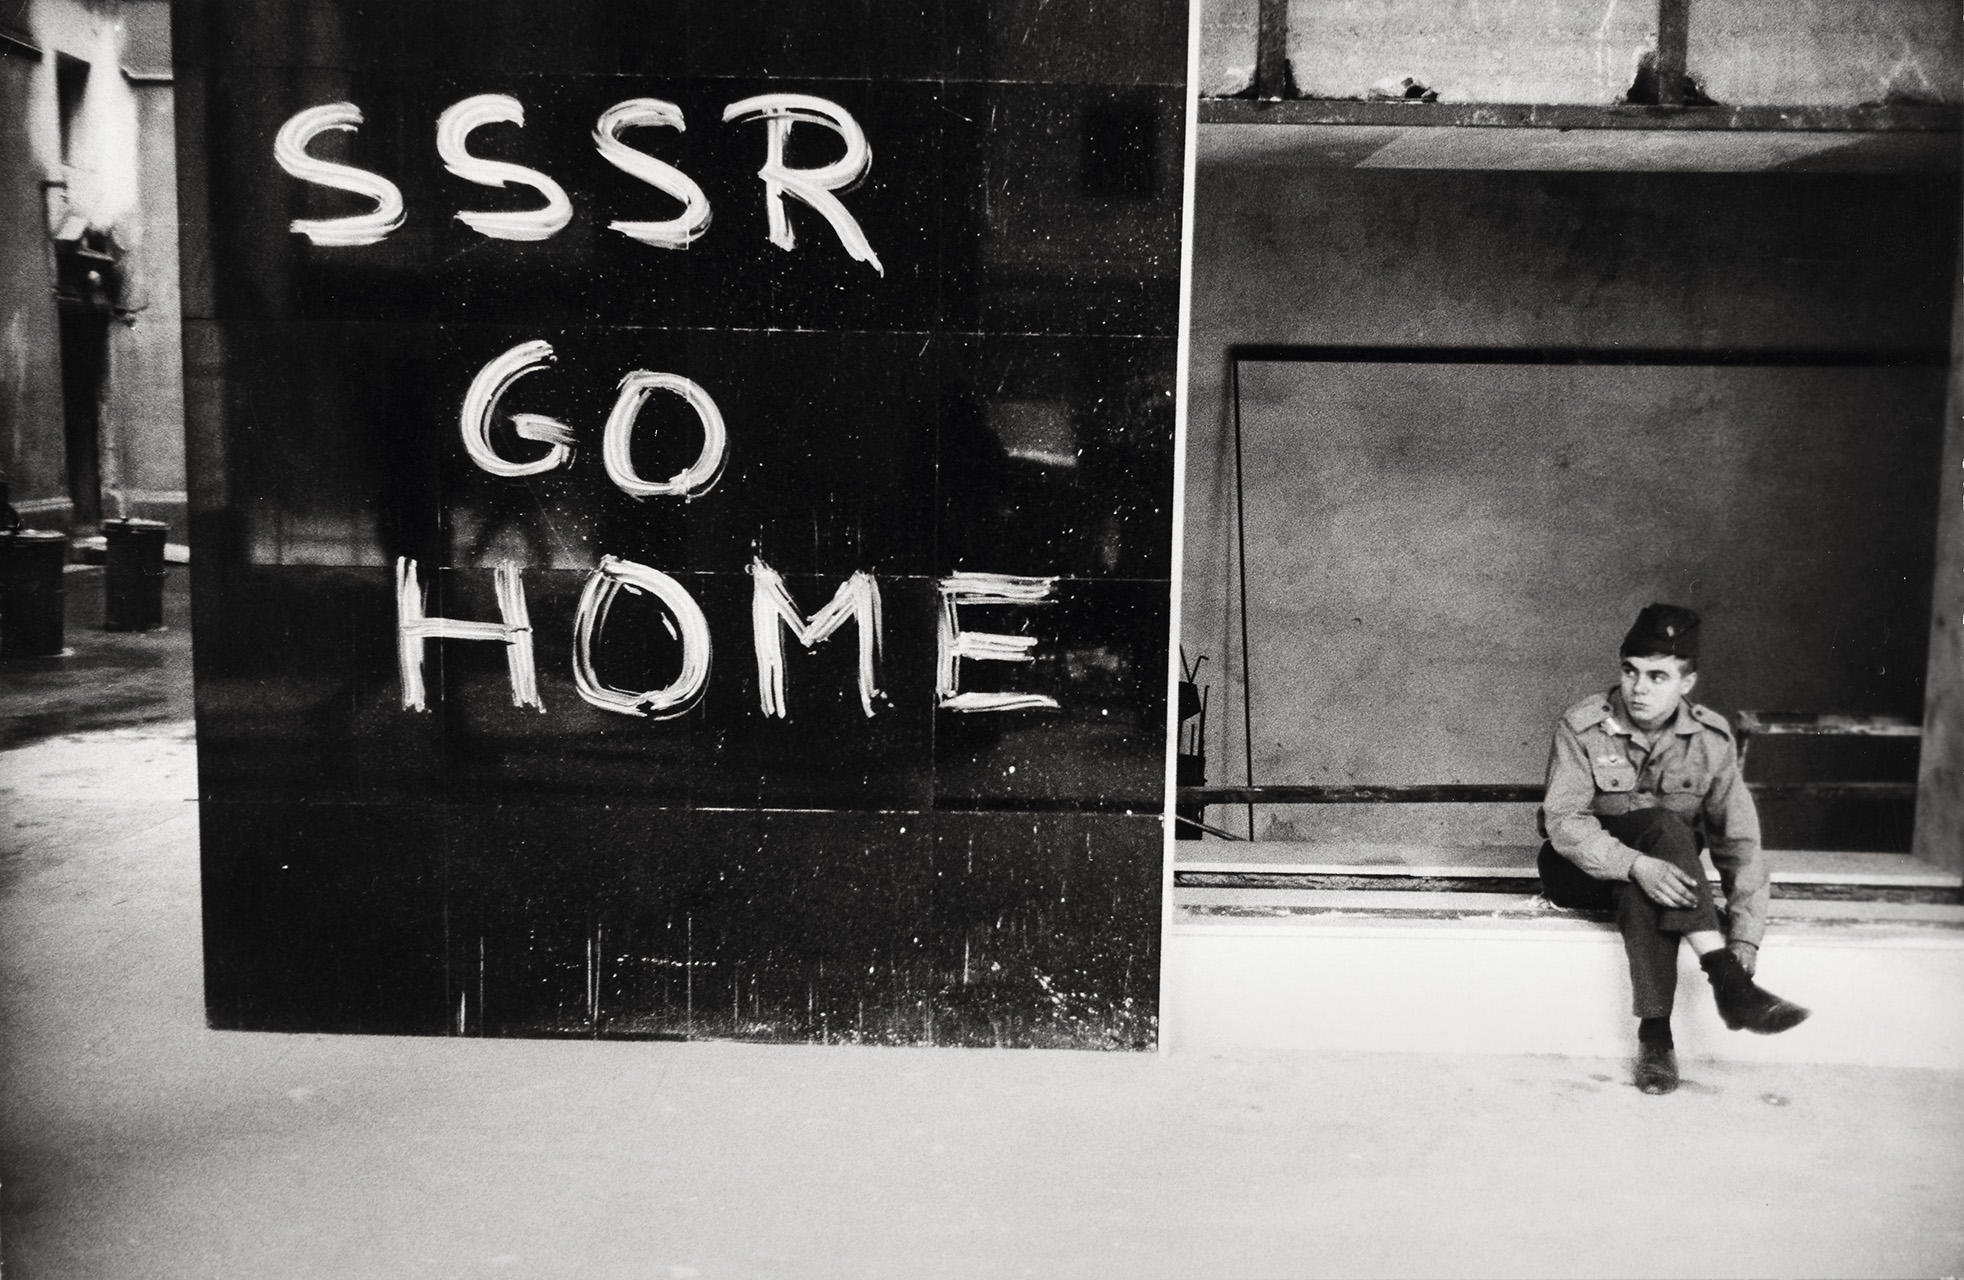
\includegraphics[width=\textwidth]{images/source_images/Ian_Berry_A young_Russian soldier.jpg}
    \caption{Ян Берри. Молодой советский солдат отдыхает рядом с плакатом <<СССР, возвращайся домой>> на Вацлавской площади. Прага, Чехословакия. 1968}
    \label{img:Soldier_orig}
\end{figure} 

Нашей задачей будет минимизация дефектов формы на надписи \textit{SSSR GO HOME}. В этом нам поможет \textit{Python}. Для начала загрузим изображение и выберем область изображения с надписью для выполения преобразований.

\begin{lstlisting}[caption={Исходный код для считывания изображения}, label={lst:img_reading}]
    # loading grayscale image
    src_img = cv.imread('source_images/Ian_Berry_A young_Russian soldier.Jpeg', 0)
    assert src_img is not None, "File could not be read"
    result = np.copy(src_img)
    # selecting specific area
    spec_area = src_img[0:735, 200:1080]
\end{lstlisting}

\begin{figure}[ht!]
    \centering
    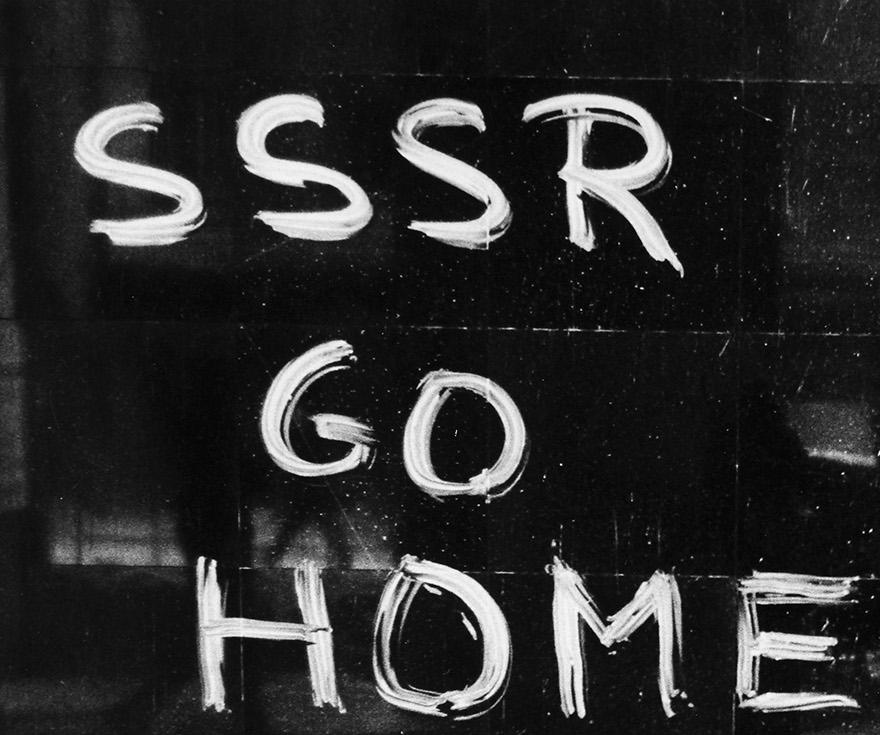
\includegraphics[width=0.7\textwidth]{images/transformed_images/1/Caption.jpg}
    \caption{Надпись, которая подвергнется преобразованиям}
    \label{img:Caption_orig}
\end{figure} 

С помощью эрозии избавимся от лишних точек на стене и выступов на буквах. Далее применим дилатацию от избавления от <<внутренних дырок>> и затем эрозию для избавления от частиц, появившихся в результате дилатации, и возвращения буквам их исходной толщины.

\begin{lstlisting}[caption={Исходный код для преобразования надписи}, label={lst:morphological}]
    # morphological operations
    disk = cv.getStructuringElement(cv.MORPH_ELLIPSE, (3, 3))
    erosion = cv.erode(spec_area, disk, iterations=1)
    dilation = cv.dilate(erosion, disk, iterations=7)
    erosion2 = cv.erode(dilation, disk, iterations=5)
\end{lstlisting}
\begin{figure}
    \centering
    \begin{subfigure}[b]{0.3\textwidth}
        \centering
        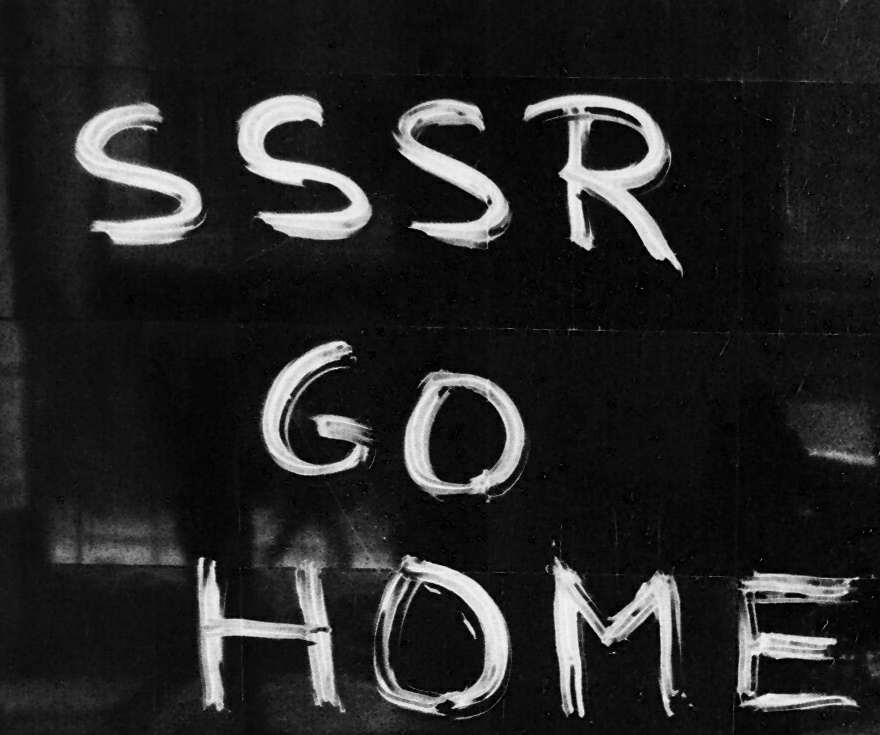
\includegraphics[width=\textwidth]{images/transformed_images/1/4 try/Erosed_1.jpg}
        \caption{}
        \label{img:Caption_erosed_1}
    \end{subfigure}
    \begin{subfigure}[b]{0.3\textwidth}
        \centering
        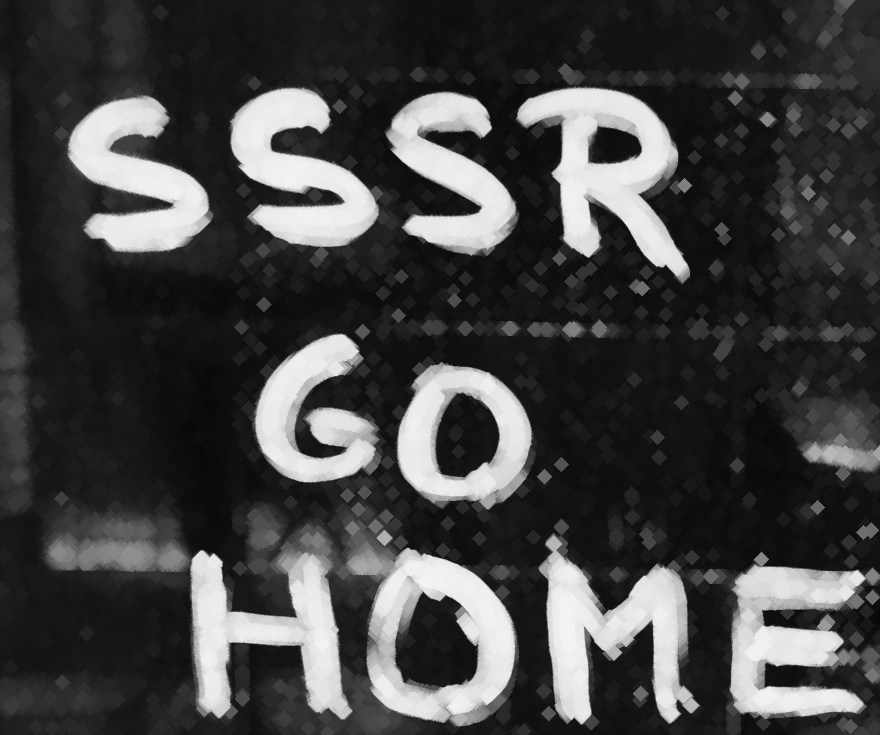
\includegraphics[width=\textwidth]{images/transformed_images/1/4 try/Dilation_7.jpg}
        \caption{}
        \label{img:Caption_dilation}
    \end{subfigure}
    \begin{subfigure}[b]{0.3\textwidth}
        \centering
        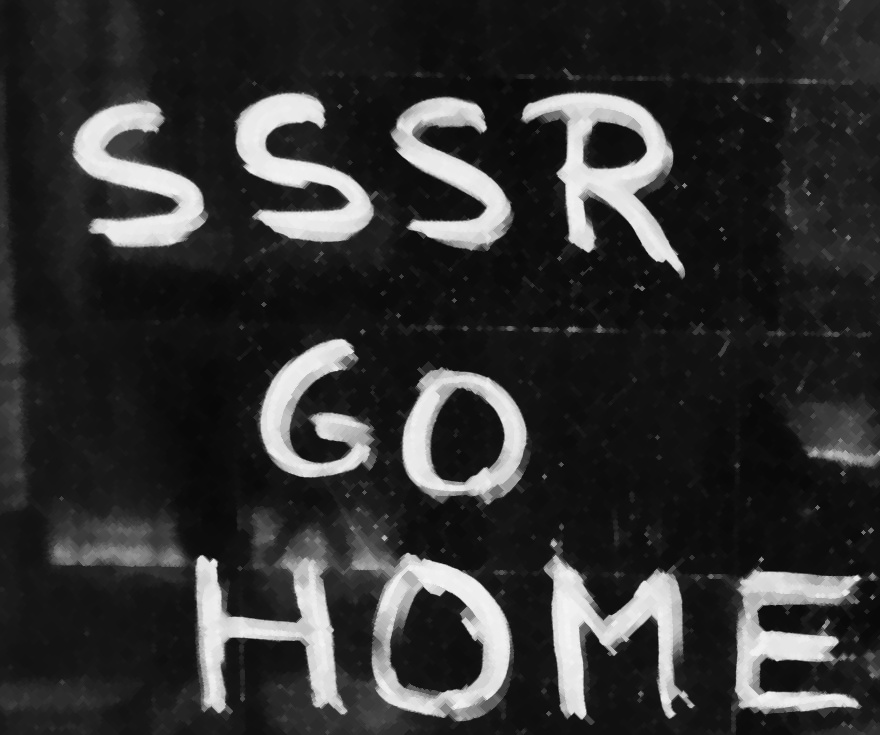
\includegraphics[width=\textwidth]{images/transformed_images/1/4 try/Erosed_2_5.jpg}
        \caption{}
        \label{img:Caption_erosed_2}
    \end{subfigure}
    \caption{Избавление от дефектов: (а) результат применения эрозии, (b)  результат применения дилатации 7 раз, (c)  результат применения эрозии 5 раз}
    \label{img:Transforms}
\end{figure}
\clearpage

\subsection{Результаты}

После преобразований необходимо вернуть <<новую>> надпись в исходное изображение.

\begin{lstlisting}[caption={Исходный код для получения итогового изображения}, label={lst:result}]
    # displaying transformed image
    result[0:735, 200:1080] = erosion2
    display_image('Result', result, 1)
\end{lstlisting}

\begin{figure}[ht!]
    \centering
    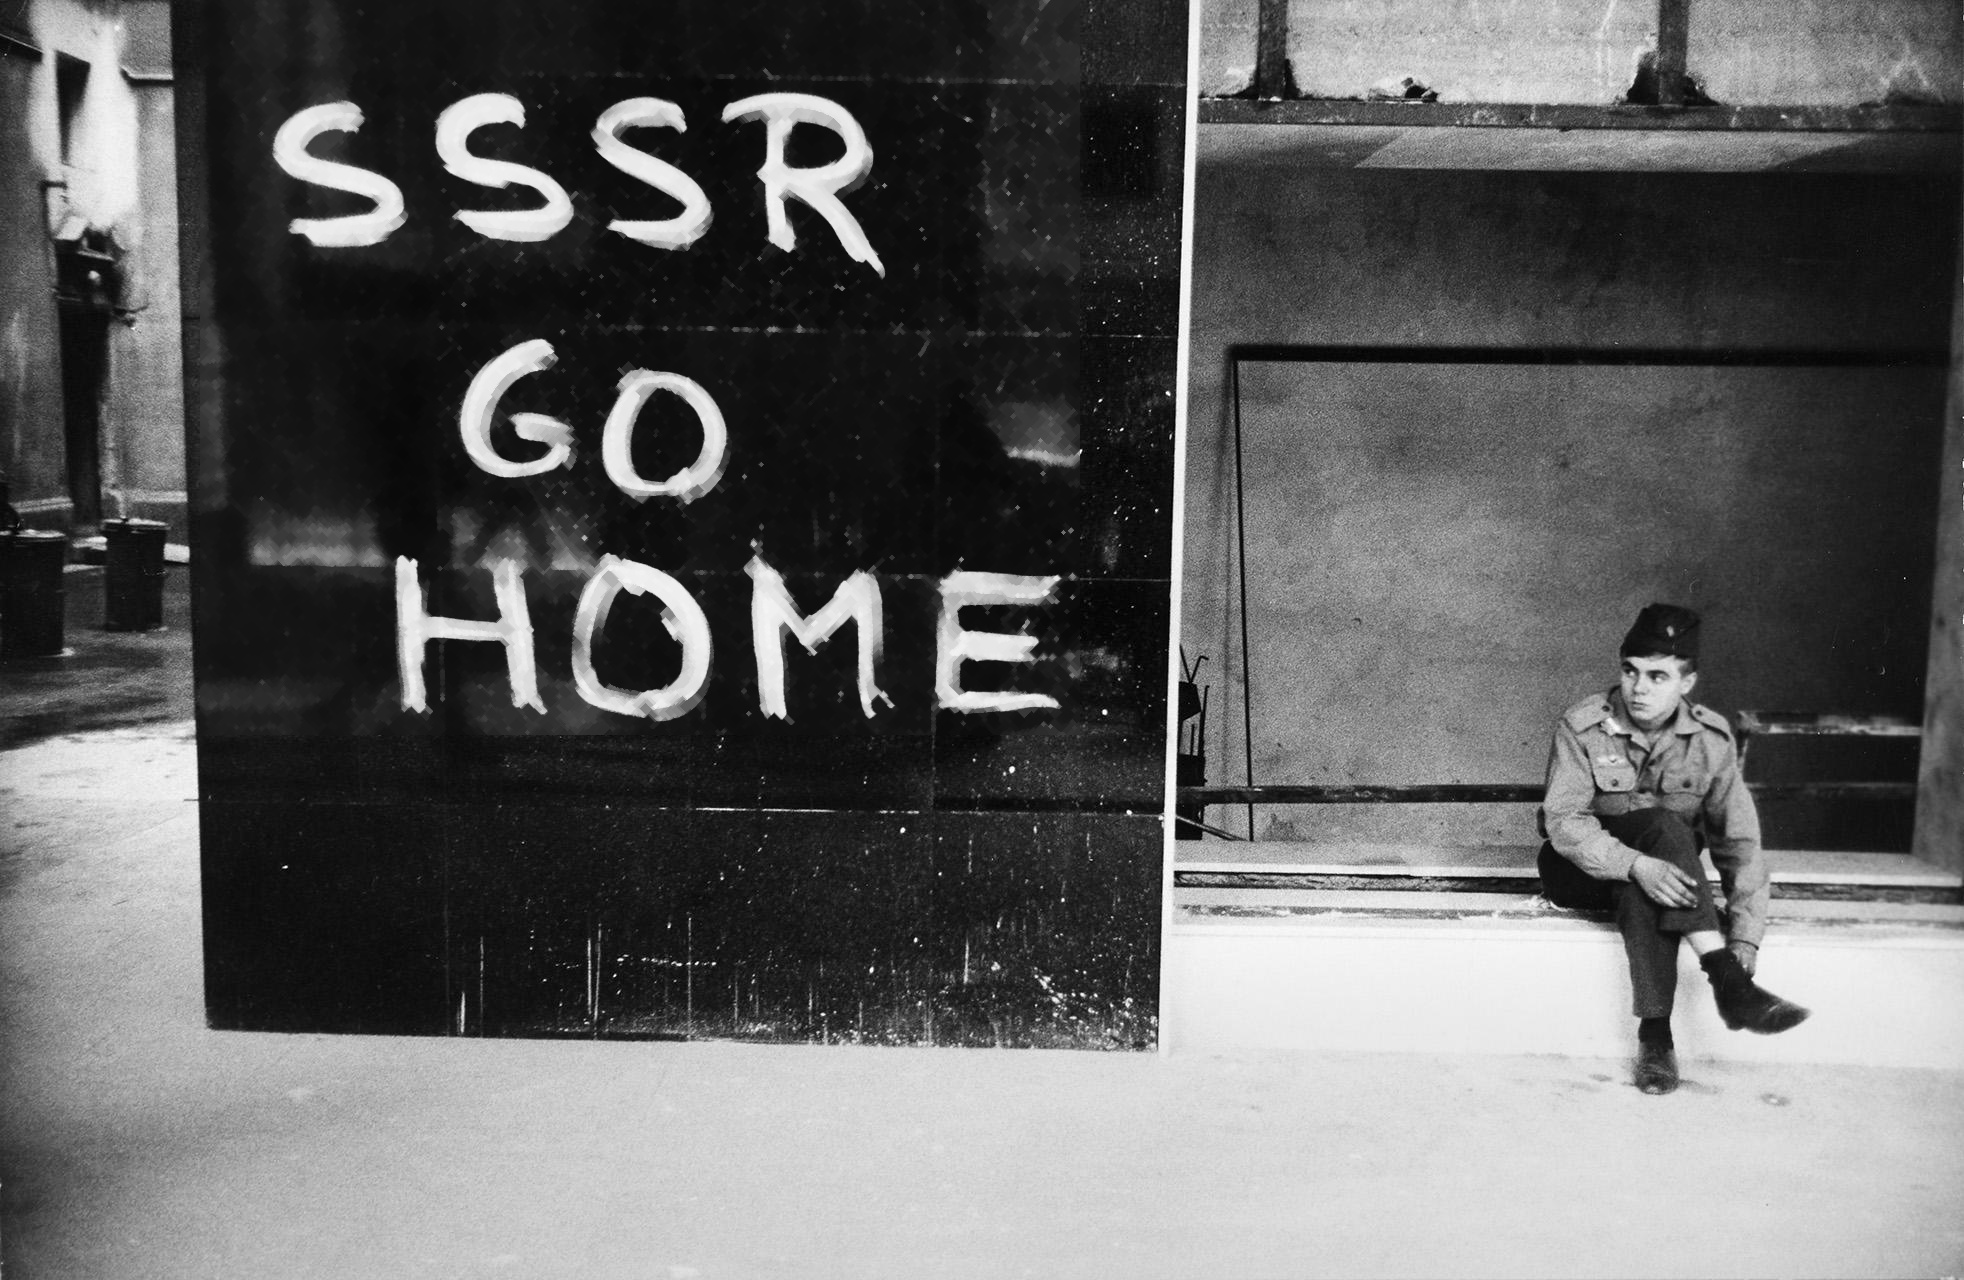
\includegraphics[width=\textwidth]{images/transformed_images/1/4 try/Result.jpg}
    \caption{Результат применения базовых морфологических операций}
    \label{img:Soldier_result}
\end{figure} 

